%%
%% UnBTeX: A class for bachelor, master, and doctoral thesis at the
%% University of Brasilia (UnB), Brazil
%% Version 1.6.6 2026/06/15
%% Copyright (C) 2021-2026 by Henrique C. Ferreira <hcferreira@unb.br>
%%
%% This class file may be distributed and/or modified under the conditions
%% of the LaTeX Project Public License, either version 1.3 of this license
%% or (at your option) any later version. The latest version of this
%% license is in:
%%
%%    https://www.latex-project.org/lppl.txt
%%
%% and version 1.3 or later is part of all distributions of LaTeX version
%% 2005/12/01 or later.
%%
%% Compile unbtex.tex with pdflatex, bibtex, and makeindex
%% (configured for the nomencl package), then run pdflatex twice more
%% (or use latexmk with the provided latexmkrc file)
%%

\documentclass[
    % -- Opções da classe memoir -- https://www.ctan.org/pkg/memoir
    oneside, % Para imprimir somente na frente da folha
    %twoside, % Para imprimir na frente e no verso da folha
    %draft, % Para compilar pela primeira vez trabalhos com timeout
    % -- Opções da classe abntex2 -- https://www.ctan.org/pkg/abntex2
    sumario=tradicional, % Sumário padrão da classe memoir
    %sumario=abnt, % Sumário padrão ABNT
    %chapter=TITLE, % Títulos dos capítulos em letras maiúsculas
    % -- Opções de idioma
    idioma=brazil, % Para texto principal em português
    %idioma=english, % Para texto principal em inglês
    % -- Opções para as referências bibliográficas
    bib=alf, % Bibliografia estilo autor-data
    %bib=num, % Bibliografia estilo numérico, com número entre [ ]
    %bib=(num), % Bibliografia estilo numérico, com número entre ( )
    %bib=overcite, % Bibliografia com números sobrescritos
    %bib=foot, % Bibliografia nas notas de rodapé
    %refbib=abnt, % Lista de referências conforme normas da ABNT
    refback, % Indica na bibliografia onde cada referência é citada
    % -- Opções de estilo de numeração de figuras, tabelas, etc.
    num=tradicional, % Numeração por capítulo
    %num=abnt, % Numeração para o documento inteiro
    ]{unbtex}

% ---
% Pacotes básicos (Adicione outros pacotes necessários para o seu trabalho)
% ---
\usepackage{lscape} % Pacote para rotacionar tabelas (e outros objetos)
%\usepackage{pdflscape} % Pacote para rotacionar objetos e também a página do arquivo pdf
\usepackage{afterpage} % Evita quebra de página quando inserir uma tabela (ou outro objeto) rotacionada
% ---

% ---
% Compila a nomenclatura
% ---
\makenomenclature
% ---

% ---
% Diretório das figuras
\graphicspath{{src/figuras/}}
% --- 

% ------------------------------------------------------------------------
% ------------------------------------------------------------------------
% INÍCIO DO DOCUMENTO
% ------------------------------------------------------------------------
% ------------------------------------------------------------------------
\begin{document}

% ------------------------------------------------------------------------
% INFORMAÇÕES DO TRABALHO
% ------------------------------------------------------------------------

% ---
% Título
% ---
\titulo{Modelo de trabalho\\ acadêmico com UnB\TeX} % No idioma principal do texto
% Insira \\ caso queira forçar quebras de linha no título
% Não utilize caixa alta para o título do trabalho e nem das seções (com exceção de siglas)
% ---
\tituloestrangeiro{} % Escreva aqui título em português se o trabalho for escrito em inglês (caso contrário, deixe vazio)
% ---

% ---
% Autores
% ---
\autori[]{Carlos}{Lisboa} % \autori[]{Nome}{Sobrenome}
% No caso de nomes como José Camargo da Costa, utilize \autori[]{José Camargo da}{Costa} (e não \autori[]{José Camargo}{da Costa})
% ---
\autorii[]{}{} % Deixe os argumentos vazios se não tiver segundo autor
% ---

% ---
% Código Cutter para a ficha catalográfica
% Gerado a partir da entrada <Sobrenome, Nome> (do primeiro autor) no site https://www.tabelacutter.com/
% ---
\numerocutter{} % Para não imprimir o código na ficha catalográfica, deixe o argumento vazio
%\numerocutter{769} % Prencher o argumento do comando apenas com os números gerados
% ---

% ---
% Orientadores
% ---
\orientador[Orientador]{Prof. Dr.}{Lourenço Nassib}{Chehab} % Para alterar o gênero, basta trocar Orientador por Orientadora
%\orientador[Orientadora]{Profa. Dra.}{Sylla Helena Ortegosa da}{Cunha}
% ---
\coorientador[Coorientador]{}{}{} % Deixe os argumentos para nome e sobrenome vazios se não tiver coorientador 
% ---

% ---
% Informações do curso
% ---
\tipotrabalho{Trabalho de Conclusão de Curso} % Dissertação de Mestrado; Tese de Doutorado (em português, mesmo que o trabalho seja em inglês)
%\tipotrabalho{Tese de Doutorado}
% ---
\tipocurso{Engenharia Elétrica} % Nome do curso de graduação ou do programa de pós-graduação, em português
%\tipocurso{Programa de Pós-Graduação em Engenharia Elétrica}
% ---
% Texto que aparece na folha de rosto e na folha de aprovação
\preambulo{Trabalho de Conclusão de Curso submetido como requisito parcial para obtenção do grau de Engenheiro Eletricista.} 
%\preambulo{Tese de Doutorado submetida ao Programa de Pós-Graduação em Engenharia Elétrica da Universidade de Brasília como parte dos requisitos necessários para obtenção do grau de Doutor.}
% Consulte a secretaria/coordenação do curso para saber o que deve ser escrito no preâmbulo. Use português mesmo que o trabalho seja em inglês.
% ---
% Informação adicional para ser impressa na folha de rosto
\publicacao{} % Deixe o argumento vazio caso não haja
%\publicacao{Publicação PPGEE 201/23} % Também imprime as informações do trabalho no topo da página da ficha catalográfica
% ---

% ---
% Instituição
% ---
%\instituicao[Universidade de Brasília]{Faculdade de Tecnologia}{} % Use português mesmo que o trabalho seja em inglês
\instituicao[Universidade de Brasília]{Faculdade de Tecnologia}{Departamento de Engenharia Elétrica} % Caso queira incluir o departamento da unidade acadêmica
% ---

% ---
% Local e data da defesa
% ---
\local{Brasília}
\dia{15}
\mes{junho}
\ano{2026}
% ---

% ---
% Membros da banca
% ---
\membrodabancai{Prof. Dr. Lourenço Nassib Chehab\\ UnB/FT/ENE} % Membro 1 - Geralmente é o orientador
\membrodabancaifuncao{Orientador} % Em português, mesmo que o trabalho seja em inglês.
\membrodabancaii{Prof. Dr. Sérgio Barroso de Assis Fonseca\\ UnB/FT/ENE} % Membro 2
\membrodabancaiifuncao{Examinador interno}
\membrodabancaiii{Prof. Dr. Nelson Ortegosa da Cunha\\ UnB/FT/ENE} % Membro 3
\membrodabancaiiifuncao{Examinador interno}
\membrodabancaiv{} % Deixe vazio se não tiver o quarto membro
\membrodabancaivfuncao{Examinador externo}
\membrodabancav{} % Deixe vazio se não tiver o quinto membro
\membrodabancavfuncao{Examinador externo}
% ---

% ---
% Resumo em português
% ---
\begin{Resumo}
Este documento exemplifica a elaboração de trabalho acadêmico (trabalho de conclusão de curso, dissertação e tese) a partir da classe UnB\TeX, uma extensão da classe abn\TeX2 para a Universidade de Brasília (UnB). Além de apresentar comandos básico de \LaTeX\ para inclusão de equações, tabelas e figuras, o documento mostra como utilizar pacotes adotados pela classe UnB\TeX\ para gerar referências bibliográficas, listas símbolos, caixas para teoremas e algoritmos, dentre outros elementos úteis ou obrigatórios para trabalhos acadêmicos. Espera-se que este documento facilite o uso da classe UnB\TeX\ na elaboração de trabalhos de alta qualidade gráfica mesmo por usuários com pouca experiência em \LaTeX.
\end{Resumo}
% ---

% ---
% Resumo em inglês
% ---
\begin{Abstract}
This document demonstrates the preparation of academic works (such as final papers, dissertations, and theses) using the UnB\TeX\ class, an extension of the abn\TeX2 class developed for the University of Brasília (UnB). In addition to introducing basic \LaTeX\ commands for the inclusion of equations, tables, and figures, the document shows how to utilize packages integrated with the UnB\TeX\ class to generate bibliographic references, lists of symbols, and formatted boxes for theorems and algorithms, among other essential or useful elements for academic writing. The goal is to simplify the use of the UnB\TeX\ class, enabling even users with minimal \LaTeX\ experience to produce visually high-quality academic documents.
\end{Abstract}
% ---

% ---
% Palavras-chave (recomenda-se de 3 a 5) separadas por vírgula
% ---
\palavraschave{
palavra-chave 1,
palavra-chave 2,
palavra-chave 3,
palavra-chave 4,
%palavra-chave 5,
}
\keywords{
keyword 1,
keyword 2,
keyword 3,
keyword 4,
%keyword 5,
}
% ---

% ---
% Agradecimentos
% ---
% Idioma usado nos agradecimentos (pode ser em português, mesmo que o trabalho seja em inglês)
\idiomaagradecimentos{brazilian}
%\idiomaagradecimentos{english}

% Primeiro autor
\begin{AgradecimentosAutorI}
Agradecemos ao Dr. Lauro César Araujo e à equipe responsável pelo desenvolvimento da classe abn\TeX2 para escrita de trabalhos acadêmicos em conformidade com as normas da ABNT. A classe UnB\TeX\ toma o abn\TeX2 como base para atender necessidades específicas de cursos de graduação e pós-graduação da Universidade de Brasília.

Agradecemos também aos usuários do fórum LaTeX Stack Exchange e do grupo de desenvolvedores do abn\TeX2. As perguntas e respostas disponíveis nesses fóruns contribuíram significativamente para a solução de diversos problemas encontrados durante o desenvolvimento da classe UnB\TeX.
\end{AgradecimentosAutorI}

% Segundo autor
\begin{AgradecimentosAutorII}
Agradecimentos do segundo autor.
\end{AgradecimentosAutorII}
% ---

% ---
% Dedicatória
% ---
% Primeiro autor
\begin{DedicatoriaAutorI}
Este trabalho é dedicado às crianças adultas que,\\
quando pequenas, sonharam em se tornar cientistas.
\end{DedicatoriaAutorI}

% Segundo autor
\begin{DedicatoriaAutorII}
Dedicatória do segundo autor.
\end{DedicatoriaAutorII}
% ---

% ---
% Epígrafe
% ---
\begin{Epigrafe}
\vspace*{\fill}
\begin{flushright}
    \textit{``If you find that you're spending almost all your time on theory,\\
    start turning some attention to practical things;\\
    it will improve your theories.\\
    If you find that you're spending almost all your time on practice,\\
    start turning some attention to theoretical things;\\
    it will improve your practice.''\\
    (Donald Knuth)}
\end{flushright}
\end{Epigrafe}
% ---

% ------------------------------------------------------------------------
% ELEMENTOS PRÉ-TEXTUAIS
% ------------------------------------------------------------------------
\pretextual

% Insere capa e contracapa
\imprimircapa

% Insere folha de rosto
\imprimirfolhaderosto*

% Insere ficha bibliográfica
\imprimirfichacatalografica

% Insere folha de aprovação
\imprimirfolhadeaprovacao

% Insere dedicatória (elemento opcional)
\imprimirdedicatoria

% Insere agradecimentos (elemento opcional)
\imprimiragradecimentos

% Insere epígrafe (elemento opcional)
\imprimirepigrafe

% Insere resumos
\imprimirresumos

% Insere lista de figuras
\imprimirlistadefiguras

% Insere lista de quadros
%\imprimirlistadequadros

% Insere lista de tabelas
\imprimirlistadetabelas

% Insere lista de algoritmos
%\imprimirlistadealgoritmos

% Insere lista de códigos
%\imprimirlistadecodigos

% Insere a lista de abreviaturas e siglas e a lista de símbolos
\imprimirlistadesiglasesimbolos

% Insere o sumário
\imprimirsumario

% ------------------------------------------------------------------------
% ELEMENTOS TEXTUAIS
% ------------------------------------------------------------------------
\textual % Cabeçalho com número da página e linha horizontal
%\textualabntex % Cabeçalho com número da página, título do capítulo/seção e linha horizontal

% Imprime uma página para agrupar um conjunto de capítulos (parte)
%\part{Nome da parte}

% Capítulo de introdução
% ----------------------------------------------------------
\chapter{Introdução}
\label{cap:intr}
% ----------------------------------------------------------

Este documento e seu código-fonte exemplificam a elaboração de trabalhos acadêmicos (trabalhos de conclusão de curso, dissertações e teses) utilizando a classe UnB\TeX, uma extensão da classe abn\TeX2 \cite{abntex2classe} desenvolvida para atender às necessidades da Universidade de Brasília (UnB).

% Definição da nomenclatura que irá para a lista de siglas e abreviações
\nomenclature[A]{UnB}{Universidade de Brasília}

O abn\TeX2, por sua vez, consiste em uma customização da classe \textsf{memoir} destinada à produção de documentos em conformidade com a ABNT NBR 14724, \emph{Informação e documentação -- Trabalhos acadêmicos -- Apresentação}. Informações sobre o projeto estão disponíveis em \url{https://www.abntex.net.br/}.

\nomenclature[A]{ABNT}{Associação Brasileira de Normas Técnicas}

A classe UnB\TeX\ foi desenvolvida com o objetivo de incorporar as atualizações das normas NBR 6023 \cite{NBR6023:2025}, NBR 10520 \cite{NBR10520:2023} e NBR 14724 \cite{NBR14724:2024}, publicadas após a descontinuação das atualizações do abn\TeX2, além de atender aos requisitos específicos dos cursos de graduação e pós-graduação da Universidade de Brasília.

Este documento deve ser utilizado como complemento à documentação do abn\TeX2 \cite{abntex2classe} e da classe \textsf{memoir} \cite{memoir}. Referências adicionais sobre \LaTeX, abn\TeX2 e assuntos correlatos podem ser encontradas em \url{https://github.com/abntex/abntex2/wiki/Referencias}.

%\begin{mdframed}[style=defnSty,innertopmargin=8pt] % azul
\begin{mdframed}[style=plainSty,innertopmargin=8pt] % verde
{\center \textsc{Texto motivador} \par}
\noindent Esperamos que o UnB\TeX\ contribua para a qualidade do seu trabalho, permitindo que sua atenção se concentre principalmente no conteúdo e na contribuição científica.
\end{mdframed}

% Capítulo de fundamentos teóricos ou técnicos
% ----------------------------------------------------------
\chapter{Comandos do \LaTeX\ e do UnB\TeX}
\label{cap:exemplos}
% ----------------------------------------------------------

Este capítulo ilustra o uso de comandos do \LaTeX\ e do UnB\TeX\ para elaboração de trabalhos acadêmicos.

% ---
\section{Opções da classe UnB\TeX}
\label{sec:opcoes}
% ---

A classe UnB\TeX\ oferece opções que permitem personalizar diferentes aspectos da formatação e da estrutura do documento. Essas opções são informadas entre colchetes no comando \texttt{\textbackslash documentclass[⟨}\emph{opções}\texttt{⟩]\{unbtex\}} do arquivo \texttt{tex} principal. Caso sejam utilizadas várias opções, elas devem ser separadas por vírgulas.

As opções da classe UnB\TeX\ são descritas ao longo dos \cref{cap:exemplos,cap:tabfig}, juntamente com os recursos correspondentes. Adicionalmente, podem ser utilizadas diversas opções da classe \textsf{memoir} \cite{memoir}, como \texttt{oneside} (impressão em um lado da folha) e \texttt{twoside} (impressão frente e verso)\footnote{As opções de tamanho de papel e fonte não estão disponíveis, pois são definidas pelas normas da ABNT.}.

% ---
\section{Expressões matemáticas}
\label{sec:mat}
% ---

Expressões matemáticas inseridas no corpo do texto, como \(\lim_{x \to \infty}\exp(-x) = 0\), devem ser delimitadas por \verb|\(...\)| (ou por \verb|$...$|). Para destacá-las em linha própria, sem numeração, utilize \verb|\[...\]|:
\[
\left|\sum_{i=1}^n a_ib_i\right|
\leq
\left(\sum_{i=1}^n a_i^2\right)^{1/2}
\left(\sum_{i=1}^n b_i^2\right)^{1/2}.
\]

O ambiente \texttt{equation} pode ser utilizado para exibir expressões matemáticas numeradas, como no exemplo a seguir:
\begin{equation}
  \forall x \in \mathcal{X}, \quad \exists \: y \leq \epsilon.
\end{equation}

Se a equação fizer parte do parágrafo, não deixe no arquivo \texttt{tex} uma linha em branco entre o texto e o ambiente da equação. A linha em branco é entendida como começo de um novo parágrafo, que é iniciado com recuo e maior espaçamento.

Muitos cientistas utilizam o \LaTeX\ devido à facilidade com que permite escrever expressões matemáticas, como:
\begin{equation}
p+\frac{1}{2}{\rho}v^2+{\rho}gh = \mathrm{constante}.
\label{eq:bernoulli}
\end{equation}
Na \cref{eq:bernoulli}, conhecida como equação de Bernoulli, $p$, $v$ e $h$ representam, respectivamente, a pressão, a velocidade e o nível em um escoamento de fluido.

% Definição da nomenclatura que irá para a lista de símbolos
\nomenclature[F]{$p$}{Pressão}
\nomenclature[F]{$v$}{Velocidade}
\nomenclature[F]{$h$}{Nível}

A seguir são apresentados mais alguns exemplos de equações feitas com o \LaTeX:

\begin{equation}\label{eq:R_f_usual}
\bm{\mathrm{R}}_r(t) = \bm{\mathrm{R}}_{\chi}(t) \triangleq 
\begin{bmatrix}
\cos \chi_0 (t) & -\sin \chi_0 (t) & 0
\\
\sin \chi_0 (t) & \cos \chi_0 (t) & 0
\\
0 & 0 & 1
\end{bmatrix},
\end{equation}

\begin{equation}
\bm{L}_{ij} = 
\begin{cases}
-a_{ij}, & \textrm{se } j \neq i \textrm{ e } j \in \mathcal{N}_i, \\
\sum_{k \in \mathcal{N}_i} a_{ik}, & \textrm{se } j = i,  \\
0, & \textrm{caso contrário},
\end{cases}
\end{equation}

\begin{equation}\label{eq:point-mass-velocity}
\begin{split}
\dot{V}_{i}(t) &{}= \frac{T_{i}(t) - D_i(t)}{m_i} - g \sin \gamma_{i}(t) + b_{ti}(t), \\
\dot{\chi}_i(t) &{}= \frac{L_i(t) \sin \phi_i(t)}{m_i V_{i}(t) \cos \gamma_{i}(t)} + \frac{b_{\psi i}(t)}{V_{i}(t)\cos \gamma_{i}(t)}, \\
\dot{\gamma}_{i}(t) &{}= \frac{L_i(t) \cos \phi_i(t)}{m_i V_{i}(t)} - \frac{g \cos \gamma_{i}(t)}{V_{i}(t)} + \frac{b_{\theta i}(t)}{V_{i}(t)}.
\end{split}
\end{equation}

\nomenclature[G]{$\theta$}{Ângulo de arfagem}
\nomenclature[G]{$\phi$}{Ângulo de rolamento}
\nomenclature[G]{$\psi$}{Ângulo de guinada}

\begin{subequations}
\begin{align}
\tau_{li}^s(t) &= \ddot{p}^d_{li}(t) - k_{d} \dot{e}_{li}(t) - k_{p} e_{li}(t), \\
\dot{\tau}_{li}^f(t) +  \xi_{i} \tau_{li}^f(t) &= u_{li}(t),\label{eq:filtro_i} \\
u_{li}(t) &= - \textrm{sign}(s_{li}(t))\eta. \label{eq:u_xbi}
\end{align}
\end{subequations}

Exemplos de fontes tipográficas específicas para uso em expressões matemáticas são apresentados na \cref{tab:ftmath}.

\begin{table}[htb]
\centering
\caption{Fontes matemáticas}
\label{tab:ftmath}
\begin{tabular}{ll}
\toprule
Exemplo & Comando \\ \midrule
$\mathcal{RQSZ}$ & \verb|\mathcal{RQSZ}| \\
$\mathscr{RQSZ}$ & \verb|\mathscr{RQSZ}| \\
$\mathfrak{RQSZ}$ & \verb|\mathfrak{RQSZ}| \\
$\mathbb{RQSZ}$ & \verb|\mathbb{RQSZ}| \\
\bottomrule
\end{tabular}
\fonte{Elaborada pelo autor}
\end{table}

% ---
\section{Lista de abreviaturas e siglas e lista de símbolos}
% ---

A lista de abreviaturas e siglas e a lista de símbolos são elementos pré-textuais opcionais de trabalhos acadêmicos. Essas listas são geradas pelo pacote \textsf{nomencl} e incluídas no documento por meio do comando \verb|\imprimirlistadesiglasesimbolos|, inserido no arquivo \texttt{tex} principal do trabalho. As entradas dessas listas são definidas conforme descrito a seguir.

Para adicionar uma entrada à lista de abreviaturas e siglas ou à lista de símbolos, utilize o comando \texttt{\textbackslash nomenclature[⟨}\emph{prefixo}\texttt{⟩]\{⟨}\emph{símbolo}\texttt{⟩\}\{⟨}\emph{descrição}\texttt{⟩\}} preferencialmente próximo à primeira ocorrência do termo ou símbolo no texto. A primeira letra do campo \emph{prefixo} determina o grupo ao qual a entrada pertence.

Por exemplo, no arquivo \texttt{capitulo1.tex}, o comando
\begin{verbatim}
\nomenclature[A]{UnB}{Universidade de Brasília}
\end{verbatim}
adiciona ao grupo \texttt{A} (sem nome definido) da lista de abreviaturas e siglas uma entrada com o símbolo ``UnB'' e a descrição ``Universidade de Brasília''. De forma análoga, no arquivo \texttt{capítulo2}, os comandos:
\begin{verbatim}
\nomenclature[F]{$p$}{Pressão}
\nomenclature[G]{$\phi$}{Ângulo de rolamento}
\end{verbatim}
adicionam à lista de símbolos as entradas correspondentes aos símbolos $p$ e $\phi$, pertencentes, respectivamente, aos grupos \texttt{F} (``Símbolos romanos'') e \texttt{G} (``Símbolos gregos''). Os grupos são apresentados em ordem alfabética de acordo com a primeira letra do campo \emph{prefixo}; assim, o grupo \texttt{F} precede o grupo \texttt{G}.

Os grupos da lista de abreviaturas e siglas podem ser personalizados mediante a inclusão, antes do comando \verb|\begin{document}|, dos seguintes comandos no arquivo principal do trabalho:
\begin{verbatim}
\renewcommand{\unbtex@abbrgroups}{,A,B,C,D,}
\renewcommand{\unbtex@abbrgroupheader}[1]{
  \IfStrEqCase{#1}{
    {A}{}
    {B}{Abreviaturas}
    {C}{Siglas}
    {D}{}
  }%
}
\end{verbatim}
Os parâmetros desses comandos podem ser modificados para definir novos grupos e seus respectivos títulos. De forma análoga, os grupos da lista de símbolos podem ser personalizados por meio dos comandos:
\begin{verbatim}
\renewcommand{\unbtex@symbolgroups}{,E,F,G,X,Z,}
\renewcommand{\unbtex@symbolgroupheader}[1]{
  \IfStrEqCase{#1}{
    {E}{}
    {F}{Símbolos romanos}
    {G}{Símbolos gregos}
    {X}{Sobrescritos}
    {Z}{Subescritos}
  }%
}
\end{verbatim}

Dentro de cada grupo, as entradas são ordenadas inicialmente pelo campo \emph{prefixo}. Assim, os comandos:
\begin{verbatim}
\nomenclature[F,h]{$h$}{Nível}
\nomenclature[F,v1]{$v$}{Velocidade}
\nomenclature[F,v2]{$\bar{v}$}{Velocidade média}
\end{verbatim}
produzem, no grupo de símbolos romanos, uma lista ordenada pelos identificadores \texttt{h}, \texttt{v1} e \texttt{v2}, resultando na sequência $h$, $v$ e $\bar{v}$. Caso o prefixo das três entradas fosse apenas \texttt{F}, a ordenação passaria a depender do campo \emph{símbolo}. Nessa situação, a entrada correspondente a $\bar{v}$ poderia aparecer antes de $h$ e $v$, pois a ordenação seria realizada com base no código \LaTeX\ utilizado para representar o símbolo, isto é, \verb|\bar{v}|. Como o primeiro caractere desse código é ``\verb|\|'', sua posição na ordenação precede a das entradas cujos símbolos começam pelas letras \texttt{h} e \texttt{v}.

Para mais informações sobre o pacote \textsf{nomencl}, consulte seu manual\footnote{Disponível em: \url{https://mirrors.ctan.org/macros/latex/contrib/nomencl/nomencl.pdf}}. Nem todos os editores \LaTeX\ executam automaticamente as etapas necessárias para gerar as listas de abreviaturas, siglas e símbolos. Para mais detalhes, consulte a \cref{sec:compilar}.

%É importante mencionar que no Overleaf, para compilar um documento com lista de abreviaturas e siglas ou lista de símbolos não é necessária nenhuma ação adicional. Em outros editores \LaTeX\ pode ser necessário compilar o documento usando usando o \texttt{pdfLaTeX}, seguido pelo \texttt{Makeindex} e pelo \texttt{pdfLaTeX} novamente. O \texttt{Makeindex} deve ser previamente configurado. No TeXstudio, por exemplo, o \texttt{Makeindex} deve ser receber a seguinte configuração\footnote{Para mais informações: \url{https://tex.stackexchange.com/questions/27824/using-package-nomencl}}:
%\begin{verbatim}
%makeindex %.nlo -s nomencl.ist -o %.nls -t %.nlg
%\end{verbatim}

% ---
\section{Sumário}\label{sec:sumario}
% ---

De acordo com a ABNT NBR 14724 \cite{NBR14724:2024}, o sumário é um elemento obrigatório de trabalhos acadêmicos. A NBR 6027 \cite{NBR6027:2012} estabelece, entre outros aspectos, que os itens do sumário devem ser numerados até o quinto nível. Para atender a essas normas, utilize a opção \texttt{sumario=abnt} da classe UnB\TeX. Caso não deseje seguir esse padrão, utilize \texttt{sumario=tradicional}.

A opção \texttt{chapter=TITLE} capitaliza os títulos de capítulos no sumário e nos cabeçalhos das páginas em que se iniciam.

% ---
\section{Referências bibliográficas}\label{sec:referencias}
% ---

Assim como a classe abn\TeX2, que conta com o pacote \textsf{abntex2cite} para formatação de referências bibliográficas conforme as normas da ABNT, a classe UnB\TeX\ disponibiliza o pacote \textsf{unbtexcite} para a mesma finalidade. Seus arquivos de estilo (extensão \texttt{bst}) foram atualizados para contemplar as versões mais recentes das normas NBR 6023 \cite{NBR6023:2025}, NBR 10520 \cite{NBR10520:2023} e NBR 14724 \cite{NBR14724:2024}. Além dos estilos autor-data e numérico, a classe inclui arquivos de estilo específicos para documentos redigidos em inglês.

Cada referência citada em arquivos \texttt{tex} deve possuir uma entrada correspondente em um arquivo de referências (extensão \texttt{bib}). Informações sobre a criação e utilização dessas entradas para diferentes tipos de documentos podem ser encontradas em \citeonline{abntex2cite,abntex2cite-alf}. O \cref{apd:cit} apresenta exemplos de uso.

A \cref{tab:bibstyle} apresenta os estilos de citação disponíveis na classe UnB\TeX. No estilo autor-data (\texttt{bib=alf}), os comandos \verb|\cite| e \verb|\citeonline| produzem, respectivamente, citações como (Silva, 2026) e Silva (2026). Nos estilos numéricos, ambos os comandos produzem o mesmo resultado: o número da referência entre colchetes (\texttt{bib=num}), entre parênteses (\texttt{bib=(num)}) ou em sobrescrito (\texttt{bib=overcite} e \texttt{bib=foot}).

\begin{table}[htb]
\centering
\caption{Estilos de citação disponíveis na classe UnB\TeX}
\label{tab:bibstyle}
\begin{tabular}{lL{5cm}L{2.2cm}} \toprule
\textbf{Opção} & \textbf{Estilo} & \textbf{Exemplo} \\ \midrule
\texttt{bib=alf} & Autor-data & Silva (2026), (Silva, 2026) \\ \addlinespace
\texttt{bib=num} & Numérico entre colchetes & [1] \\ \addlinespace
\texttt{bib=(num)} & Numérico entre parênteses & (1) \\ \addlinespace
\texttt{bib=overcite} & Numérico sobrescrito & $^{1}$ \\ \addlinespace
\texttt{bib=foot} & Numérico sobrescrito com referências em rodapé & $^{1}$ \\ \bottomrule
\end{tabular}
\fonte{Elaborada pelo autor}
\end{table}

Na opção \texttt{bib=foot}, as referências são apresentadas como notas de rodapé na página em que são citadas\footnote{Em trabalhos que utilizam o sistema numérico com referências em notas de rodapé, a ABNT NBR 10520 não recomenda o uso de notas de rodapé para outras finalidades.}. Nas demais opções, as referências são reunidas em uma lista antes dos apêndices e anexos (quando existentes), contendo todas as obras citadas ao longo do documento.
% Além disso, cada apêndice ou anexo que contenha citações possui sua própria lista de referências, conforme requerido pela NBR 14724 \cite[p. 9]{NBR14724:2024}.
%Added reference lists at the end of each appendix or annex with citations, as required by NBR 14724:2024, p. 9.

Segundo a NBR 6023 \cite[p. 5]{NBR6023:2025}, a lista de referências deve ser elaborada em espaço simples, alinhada à margem esquerda e separada por uma linha em branco de espaço simples. Para seguir essa norma, utilize a opção \texttt{refbib=abnt}. A opção \texttt{refbib=tradicional}, adotada como padrão da classe UnB\TeX, utiliza o mesmo espaçamento do texto e alinhamento justificado.

A opção \texttt{refback} inclui, na lista de referências, as páginas em que cada obra é citada. Para desabilitar esse recurso, basta omitir a opção.

%-
\subsection{Acentuação de referências bibliográficas}
%-

Normalmente não há problemas em utilizar caracteres acentuados em arquivos bibliográficos (\texttt{bib}). Entretanto, como as normas da ABNT frequentemente exigem a conversão de textos para letras maiúsculas, a codificação apresentada na \cref{tab:acentos} deve ser utilizada para evitar problemas nessa conversão, especialmente em nomes de autores.

\begin{table}[htb]
\centering
\caption{Tabela de conversão de acentuação}
\label{tab:acentos}
\begin{tabular}{llllllll} \toprule
\multicolumn{4}{l}{acento} & \multicolumn{4}{l}{bibtex} \\ \midrule
\`a & \'a & \~a & \^a & \verb|{\`a}| & \verb|{\'a}| & \verb|{\~a}| & \verb|{\^a}| \\
\'e & \^e & & & \verb|{\'e}| & \verb|{\^e}| & & \\
\'i & & & & \verb|{\'i}| & & & \\
\'o & \~o & \^o & & \verb|{\'o}| & \verb|{\~o}| & \verb|{\^o}| & \\
\'u & & & & \verb|{\'u}| & & & \\
{\c c} & & & & \verb|{\c c}| & & & \\ \bottomrule
\end{tabular}
\fonte{Adaptada de \citeonline{abntex2cite}}
\end{table}

% ---
\section{Citações diretas}\label{sec:citacao}
% ---

Utilize o ambiente \texttt{citacao} para incluir citações diretas com mais de três linhas:
\begin{citacao}
A citação direta, com mais de três linhas, deve ser destacada com recuo padronizado em relação à margem esquerda, com letra menor que a utilizada no texto, em espaço simples e sem aspas. Recomenda-se o recuo de 4 cm \cite[p. 12]{NBR10520:2023}.
\end{citacao}

Use o ambiente assim:
\begin{verbatim}
\begin{citacao}
A citação direta, com mais de três linhas, deve ser destacada com recuo padronizado em 
relação à margem esquerda, com letra menor que a utilizada no texto, em espaço simples e 
sem aspas. Recomenda-se o recuo de 4 cm \cite[p. 12]{NBR10520:2023}.
\end{citacao}
\end{verbatim}

O ambiente \texttt{citacao} pode receber como parâmetro opcional um nome de idioma previamente carregado nas opções da classe UnB\TeX. Nesse caso, o texto da citação é automaticamente escrito em itálico e a hifenização (conforme comentado na \cref{sec:hifenizacao}) é ajustada para o idioma selecionado na opção do ambiente. Por exemplo:
\begin{verbatim}
\begin{citacao}[english]
Text in English language in italic with correct hyphenation.
\end{citacao}
\end{verbatim}
tem como resultado:
\begin{citacao}[english]
Text in English language in italic with correct hyphenation.
\end{citacao}

Citações simples, com até três linhas, devem ser incluídas com aspas. Observe que em \LaTeX\ as aspas iniciais são diferentes das finais: ``Amor é fogo que arde sem se ver''.

% ---
\section{Remissões internas}
% ---

Ao nomear a \cref{sec:mat} e a \cref{eq:bernoulli}, apresentamos um exemplo de remissão interna, que também pode ser feita quando indicamos o \cref{cap:exemplos}, intitulado \emph{\nameref{cap:exemplos}}. O número do capítulo indicado é \ref{cap:exemplos}, que se inicia à \cpageref{cap:exemplos}\footnote{O número da página de uma remissão pode ser obtida também assim: \pageref{cap:exemplos}.}.

O código usado para produzir o texto do parágrafo anterior é:
\begin{verbatim}
Ao nomear a \cref{sec:mat} e a \cref{eq:bernoulli}, apresentamos um exemplo de remissão
interna, que também pode ser feita quando indicamos o \cref{cap:exemplos}, intitulado
\emph{\nameref{cap:exemplos}}. O número do capítulo indicado é \ref{cap:exemplos}, que se
inicia à \cpageref{cap:exemplos}\footnote{O número da página de uma remissão pode ser
obtida também assim: \pageref{cap:exemplos}.}.
\end{verbatim}

As remissões internas neste documento foram feitas utilizando-se o pacote \textsf{cleveref}. Mais opções de uso (e de comandos) podem ser encontradas em seu manual\footnote{Disponível em: \url{https://mirrors.ctan.org/macros/latex/contrib/cleveref/cleveref.pdf}}.

A NBR 14724 \cite[p. 8]{NBR14724:2024} estabelece que trabalhos acadêmicos devem ser organizados em seções, e não em capítulos. Para atender a essa recomendação, utilize a opção \texttt{chapnamesec} da classe UnB\TeX, que substitui ``capítulo'' por ``seção'' nas remissões internas geradas pelo pacote \textsf{cleveref}.

% ---
\section{Enumerações: alíneas e subalíneas}
% ---

Quando for necessário enumerar os diversos assuntos de uma seção que não possua título, esta deve ser subdividida em alíneas \cite[p. 3]{NBR6024:2012}:

\begin{alineas}

  \item os diversos assuntos que não possuam título próprio, dentro de uma mesma seção, devem ser subdivididos em alíneas; 
  \item o texto que antecede as alíneas termina em dois pontos;
  \item as alíneas devem ser indicadas alfabeticamente, em letra minúscula, seguida de parêntese. Utilizam-se letras dobradas, quando esgotadas as letras do alfabeto;
  \item as letras indicativas das alíneas devem apresentar recuo em relação à margem esquerda;
  \item o texto da alínea deve começar por letra minúscula e terminar em ponto-e-vírgula, exceto a última alínea que termina em ponto final;
  \item o texto da alínea deve terminar em dois pontos, se houver subalínea;
  \item a segunda e as seguintes linhas do texto da alínea começa sob a primeira letra do texto da própria alínea;
  \item subalíneas \cite[p. 4]{NBR6024:2012} devem ser conforme as alíneas a seguir:

  \begin{alineas}
     \item as subalíneas devem começar por travessão seguido de espaço;
     \item as subalíneas devem apresentar recuo em relação à alínea;
     \item o texto da subalínea deve começar por letra minúscula e terminar em ponto-e-vírgula. A última subalínea deve terminar em ponto final, se não houver alínea subsequente;
     \item a segunda e as seguintes linhas do texto da subalínea começam sob a primeira letra do texto da própria subalínea.
  \end{alineas}
  
  \item no abn\TeX2 estão disponíveis os ambientes \texttt{incisos} e \texttt{subalineas} que, em suma, são o mesmo que se criar outro nível de \texttt{alineas}, como nos exemplos à seguir:
  
  \begin{incisos}
    \item \textit{Um novo inciso em itálico};
  \end{incisos}
  
  \item Alínea em \textbf{negrito}:
  
  \begin{subalineas}
    \item \textit{Uma subalínea em itálico};
    \item \underline{\textit{Uma subalínea em itálico e sublinhado}}; 
  \end{subalineas}
  
  \item Última alínea com \emph{ênfase}.
  
\end{alineas}

% ---
\section{Notas de rodapé}
% ---

A NBR 14724 \cite[p. 10]{NBR14724:2024} apresenta as diretrizes para notas de rodapé\footnote{Quando várias notas de rodapé são inseridas em sequência, os números sobrescritos são separados por vírgulas no corpo do texto.}\footnote{Verifique se os números sobrescritos aparecem separados por vírgulas no corpo do texto.}.

% ---
\section{Diferentes idiomas e hifenizações}
\label{sec:hifenizacao}
% ---

O idioma principal do texto é definido no início do arquivo \texttt{tex} principal, como uma opção da classe UnB\TeX. Para português-brasileiro, utilize a opção \texttt{idioma=brazil} e para inglês, utilize a opção \texttt{idioma=english}. A opção de idioma define se nome das listas (de figuras, de tabelas, de abreviaturas e siglas, de símbolos), do sumário e das referências será em português ou inglês. Define também o idioma do rótulo das tabelas, figuras, equações, capítulos, seções, apêndices, anexos, etc. Mesmo que o idioma principal do texto seja português, é possível incluir textos para serem hifenizados em inglês, como no exemplo a seguir\footnote{Extraído de: \url{https://en.wikibooks.org/wiki/LaTeX/Internationalization}}:

\begin{otherlanguage*}{english}
\textit{Text in English language. This environment switches all language-related definitions, like the language specific names for figures, tables etc. to the other language. The starred version of this environment typesets the main text according to the rules of the other language, but keeps the language specific string for ancillary things like figures, in the main language of the document. The environment hyphenrules switches only the hyphenation patterns used; it can also be used to disallow hyphenation by using the language name `nohyphenation'.}
\end{otherlanguage*}

A \cref{sec:citacao} descreve o ambiente \texttt{citacao}, que pode receber como parâmetro um idioma a ser usado para hifenização da citação.

% ---
\section{Ficha catalográfica com código Cutter-Sanborn}
% ---

A ficha catalográfica é um elemento pré-textual obrigatório em teses, dissertações e trabalhos de conclusão de curso. Mais informações podem ser encontradas no site da Biblioteca Central da UnB\footnote{\url{https://bce.unb.br/elaboracao-de-fichas-catalograficas/}}. A classe UnB\TeX\ gera automaticamente a ficha catalográfica a partir dos dados do trabalho, com opção de inclusão do código Cutter.

O código Cutter é obtido a partir da Tabela Cutter-Sanborn, desenvolvida por Charles A. Cutter e posteriormente expandida por Kate F. Sanborn. Ferramentas para sua obtenção estão disponíveis em diversos sites\footnote{\url{https://www.tabelacutter.com/}}\footnote{\url{https://cuttersonline.com.br/registrador-gratuito}}.

Para gerar o código, informe na ferramenta o sobrenome seguido dos prenomes do primeiro autor. Por exemplo, para Carlos Lisboa, utilize:
\begin{verbatim}
Lisboa, Carlos
\end{verbatim}
O código gerado é \texttt{769}. No arquivo \texttt{tex} principal, informe apenas os números:
\begin{verbatim}
\numerocutter{769}
\end{verbatim}
Na ficha catalográfica será exibido \texttt{L769m}, em que a letra inicial do sobrenome do autor (\texttt{L}, de \emph{Lisboa}) e a inicial do título do trabalho (\texttt{m}, de \emph{Modelo de trabalho acadêmico com UnB\TeX}) são acrescentadas automaticamente. De modo análogo, para José Camargo da Costa, utilize:
\begin{verbatim}
Costa, José Camargo da
\end{verbatim}

Caso não deseje incluir o código Cutter na ficha catalográfica, deixe o comando vazio:
\begin{verbatim}
\numerocutter{}
\end{verbatim}

% ---
\section{Inclusão de outros arquivos}\label{sec:include}
% ---

É uma boa prática dividir documentos extensos em vários arquivos, em vez de concentrar todo o conteúdo em um único arquivo. Para incluir um arquivo em outro e iniciar seu conteúdo em uma nova página, utilize o comando:
\begin{verbatim}
\include{documento-a-ser-incluido}      % sem a extensão .tex
\end{verbatim}

Para incluir um arquivo sem forçar uma quebra de página, utilize:
\begin{verbatim}
\input{documento-a-ser-incluido}        % sem a extensão .tex
\end{verbatim}

Também é possível incluir páginas de arquivos \texttt{pdf}. No \cref{anx:coresunb}, por exemplo, foi inserida uma página do manual de identidade visual da UnB utilizando o comando \verb|\includepdf| do pacote \textsf{pdfpages}. Para mais informações, consulte o manual do pacote\footnote{Disponível em: \url{https://mirrors.ctan.org/macros/latex/contrib/pdfpages/pdfpages.pdf}}.

% ---
\section{Como compilar o documento}\label{sec:compilar}
% ---

Para gerar corretamente listas de referências, listas de símbolos, remissões internas e outros elementos do documento, é necessário executar, nesta ordem, \texttt{pdfLaTeX}, \texttt{BibTeX}, \texttt{MakeIndex} e mais duas execuções do \texttt{pdfLaTeX}. O \texttt{MakeIndex} deve ser previamente configurado conforme o editor \LaTeX\ utilizado\footnote{Para TeXstudio, consulte: \url{https://tex.stackexchange.com/questions/27824/using-package-nomencl}}.

No Overleaf, esse processo é automatizado. Entretanto, devido às limitações de tempo de compilação da versão gratuita, o arquivo \texttt{latexmkrc} fornecido com o UnB\TeX\ limita a duas as execuções automáticas do \texttt{pdfLaTeX}. Assim, quando o projeto é aberto pela primeira vez, normalmente é necessário compilar o documento duas vezes para que todas as referências e listas sejam geradas corretamente.

Caso o tempo de compilação continue elevado ou uma versão paga do Overleaf esteja disponível, o arquivo \texttt{latexmkrc} pode ser ajustado para reduzir ou aumentar o número de execuções do \texttt{pdfLaTeX}. Alternativamente, pode-se utilizar a opção \texttt{draft} da classe UnB\TeX, que desabilita temporariamente o carregamento de imagens e reduz o tempo da primeira compilação.

O arquivo \texttt{latexmkrc} também automatiza a compilação em instalações locais de \LaTeX. Nessa configuração, ele está ajustado para executar o \texttt{pdfLaTeX} até quatro vezes, o que normalmente é suficiente para gerar o documento completo. No TeXstudio, por exemplo, basta selecionar \texttt{Ferramentas > Comandos > Latexmk}.

% ---
\section{Consulte o manual da classe abn\TeX2}
% ---

Consulte o manual da classe \textsf{abntex2} \cite{abntex2classe} para uma descrição completa dos comandos e ambientes disponíveis. O manual também contém informações adicionais sobre as normas da ABNT adotadas pelo abn\TeX2 e suas limitações.

% Capítulo com a proposta desenvolvida
% ----------------------------------------------------------
\chapter{Tabelas e figuras}
\label{cap:tabfig}
% ----------------------------------------------------------

A classe UnB\TeX\ permite numerar tabelas, figuras, equações, códigos, algoritmos, definições, teoremas e outros elementos por capítulo, por meio da opção \texttt{num=tradicional}, ou de forma consecutiva em todo o documento, por meio da opção \texttt{num=abnt}. Este documento adota a numeração por capítulo, embora a ABNT recomende a numeração consecutiva.

% ---
\section{Tabelas}
% ---

As \cref{tab:nivel,tab:fluxo,tab:ibge} são exemplos de tabelas construídas com \LaTeX. Observe que a \cref{tab:ibge} utiliza o padrão do \citeonline{ibge1993}, indicada pela ABNT para trabalhos acadêmicos. Neste padrão, o texto da legenda, incluído na parte superior, e os demais textos (fonte e notas), incluídos na parte inferior, têm a mesma largura da tabela.

\begin{table}[htb]
%\begin{quadro}[htb]
\centering
\small
\caption{Níveis de investigação}
\label{tab:nivel}
{\renewcommand{\arraystretch}{1.3}% espaçamento entre as linhas da tabela
\begin{tabular}{p{2.6cm}p{5.5cm}p{2.8cm}p{2.5cm}}
  \rowcolor{verdeunb!10}\textbf{Nível de Investigação} & \textbf{Insumos} & \textbf{Sistemas de Investigação} & \textbf{Produtos} \\ \hline
  Meta-nível & Filosofia da Ciência & Epistemologia & Paradigma \\ \hline
  Nível do objeto & Paradigmas do metanível e evidências do nível inferior & Ciência  & Teorias e modelos \\ \hline
  Nível inferior & Modelos e métodos do nível do objeto e problemas do nível inferior & Prática & Solução de problemas \\
\end{tabular}}
\fonte{\citeonline{gigch1986}}
%\end{quadro}
\end{table}

%\afterpage{% Evita quebra de página ao inserir tabela rotacionada
%\begin{landscape}% Rotaciona a tabela
\begin{table}
\small
\centering
\caption{Componentes curriculares do segundo nível}
\label{tab:fluxo}
{\renewcommand{\arraystretch}{1.3}% espaçamento entre as linhas da tabela
\begin{tabular}{|l|m{4.5cm}|C{.7cm}|C{.7cm}|C{.7cm}|C{.75cm}|C{.7cm}|l|}
\hline%
\multicolumn{8}{|l|}{\textbf{2º Nível}} \\ \hline%
\multirow{2}{*}{Código} &
\multirow{2}{*}{Componente curricular} &
\multicolumn{5}{c|}{Quantidade de horas} & 
\multirow{2}{*}{Pré-requisito} \\ 
\cline{3-7} & & Teo. & Pr. & Ext. & EaD & Tot. & \\ \hline\hline%
MAT0026 & Cálculo 2 & 60 & 30 & 0 & 0 & 90 & MAT0025 \\ \hline%
IFD0171 & Física 1 & 60 & 0 & 0 & 0 & 60 & \\ \hline%
IFD0173 & Física 1 Experimental & 0 & 30 & 0 & 0 & 30 & \\ \hline%
EST0023 & Probabilidade e Estatística & 30 & 30 & 0 & 0 & 60 & MAT0025 \\ \hline%
ENM0190 & Desenho Mecânico para Engenharia & 30 & 30 & 0 & 0 & 60 & \\ \hline%
CIC0090 & Estruturas de Dados & 30 & 30 & 0 & 0 & 60 & CIC0004 \\ \hline%
\multicolumn{6}{|l|}{Componentes optativos ou eletivos} & 60 & \multicolumn{1}{r}{} \\ \cline{1-7}%
\multicolumn{6}{|l|}{Total de horas do 2º Nível} & 420 & \multicolumn{1}{r}{} \\ \cline{1-7}%
\end{tabular}}
\fonte{Elaborada pelo autor}
\end{table}
%\end{landscape}
%}

\begin{table}[htb]
\centering
\IBGEtab{%
  \caption{Um Exemplo de tabela conforme o padrão IBGE}%
  \label{tab:ibge}
}{%
  \begin{tabular}{@{}ccc@{}}% @{} elimina o espaço nas bordas laterais
  \toprule
  \textbf{Nome} & \textbf{Nascimento} & \textbf{Documento}$^\ast$ \\ \midrule
  Maria da Silva & 11/11/1111 & 111.111.111-11 \\[3pt]
  João Souza & 11/11/2111 & 211.111.111-11 \\[3pt]
  Laura Vicuña & 05/04/1891 & 3111.111.111-11 \\ \bottomrule
  \end{tabular}%
}{%
  \fonte{Elaborada pelo autor}%
  \legend[Nota:]{Esta é uma nota, que diz que os dados são baseados na regressão linear}%
  \legend[$^\ast$]{Outro tipo de nota}
}
\end{table}

Para alterar cores em tabelas, foi utilizado o pacote \textsf{colortbl}. A mesclagem de linhas e colunas, exemplificada na \cref{tab:fluxo}, foi realizada com o pacote \textsf{multirow}. Sempre que possível, evite linhas verticais entre colunas. Nas \cref{tab:nivel,tab:ibge}, por exemplo, foram utilizados os comandos \verb|\toprule|, \verb|\midrule| e \verb|\bottomrule| do pacote \textsf{booktabs}, enquanto a \cref{tab:fluxo} utiliza linhas verticais e o comando \verb|\hline|. O espaçamento entre linhas pode ser ajustado com \verb|\arraystretch| e \verb|\addlinespace|.

Os pacotes \textsf{longtable} e \textsf{rotating} permitem criar, respectivamente, tabelas com múltiplas páginas e tabelas rotacionadas; exemplos podem ser encontrados no \cref{apd:tabs}. Os pacotes \textsf{tabularray} e \textsf{nicematrix} não foram utilizados neste documento devido ao maior tempo de processamento. Além disso, existem ferramentas online para gerar código \LaTeX\ para tabelas\footnote{Por exemplo: \url{https://www.tablesgenerator.com/}}.

As normas da ABNT também preveem o uso de quadros. Em geral, tabelas são utilizadas para dados numéricos e quadros para informações textuais. Para criar quadros, utilize o ambiente \texttt{quadro}, disponibilizado pela classe UnB\TeX. As listas de tabelas e quadros podem ser geradas, respectivamente, pelos comandos \verb|\imprimirlistadetabelas| e \verb|\imprimirlistadequadros|.

% ---
\section{Figuras}
% ---

Para diagramas, gráficos e ilustrações produzidos pelo próprio autor, recomenda-se o uso de imagens vetoriais em formato \texttt{pdf}, como na \cref{fig:blockdiag1}, pois permitem redimensionamento sem perda de qualidade e geralmente resultam em arquivos menores. O \textsf{InkScape} (\url{https://inkscape.org/}) é uma alternativa livre ao CorelDraw e ao Adobe Illustrator para produzir esse tipo de imagem.

\begin{figure}[htb]
\centering
\caption{Sistema em malha fechada, com realimentação da saída}
\label{fig:blockdiag1}
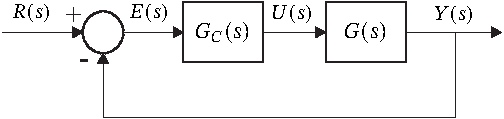
\includegraphics[scale=1]{blockdiagram.pdf}
\fonte{Elaborada pelo autor}
\end{figure}

Quando não for possível utilizar imagens em formato \texttt{pdf}, podem ser empregados formatos como \texttt{jpeg}, \texttt{gif} e \texttt{bmp}, embora normalmente resultem em maior tempo de processamento. Para editar esse tipo de imagem, uma alternativa livre ao Adobe Photoshop é o \textsf{Gimp} (\url{https://www.gimp.org/}). Figuras, diagramas e gráficos também podem ser produzidos diretamente em \LaTeX\ com pacotes como \textsf{TikZ}, que não foram utilizados neste documento por exigirem maior tempo de compilação.

De acordo com as normas da ABNT, a legenda de figuras e tabelas (comando \verb|\caption|) deve ser posicionada na parte superior, enquanto a fonte e eventuais notas (comandos \verb|\fonte| e \verb|\legend|) devem aparecer na parte inferior. Referências não devem ser incluídas na legenda superior; para isso, utilize os comandos \verb|\fonte| e \verb|\legend|. Caso deseje posicionar a legenda abaixo da figura, insira o comando \verb|\caption| após \verb|\includegraphics|. Observe ainda que, diferentemente da \cref{fig:blockdiag1}, a \cref{fig:blockdiag2} apresenta legenda e nota com a mesma largura da figura, conforme recomendado pela ABNT.

A lista de figuras pode ser incluída como elemento pré-textual por meio do comando \verb|\imprimirlistadefiguras| no arquivo \texttt{tex} principal.

\begin{figure}[htb]
\centering
\IBGEtab{%
  \caption{Digrama de blocos de sistema de controle em malha fechada}%
  \label{fig:blockdiag2}
}{%
  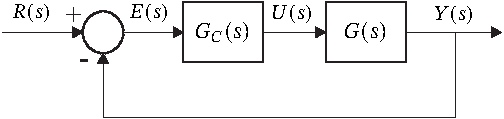
\includegraphics[scale=1]{blockdiagram.pdf}
}{%
  \fonte{Elaborada pelo autor}%
}
\end{figure}

% ---
\subsection{Figuras em \emph{minipages}}
% ---

\emph{Minipages} são usadas para inserir textos ou outros elementos em quadros com tamanhos e posições controladas. Veja os exemplos das \cref{fig:minipage_circuito,fig:minipage_grafico}.

\begin{figure}[htb]
\label{fig:teste}
\centering
\begin{minipage}[t]{0.46\textwidth}
  \centering
  \caption{Imagem da minipage}
  \label{fig:minipage_circuito}
  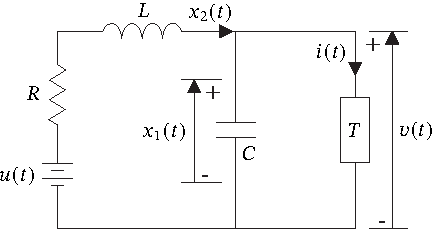
\includegraphics[scale=1]{circuito.pdf} 
  \fonte{Elaborada pelo autor}
\end{minipage}
\hfill
\begin{minipage}[t]{0.52\textwidth}
  \centering
  \caption{Gráfico da minipage}
  \label{fig:minipage_grafico}
  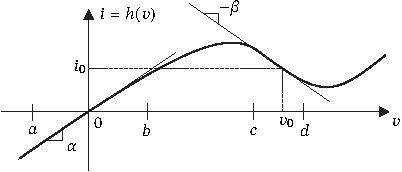
\includegraphics[scale=1.2]{diodocurva.pdf}
  \fonte{Elaborada pelo autor}
\end{minipage}
\end{figure}

%\begin{figure}[htb]
%\centering
%\captionbox{Imagem da minipage\label{fig:minipage_circuito}}
%  [0.47\textwidth]{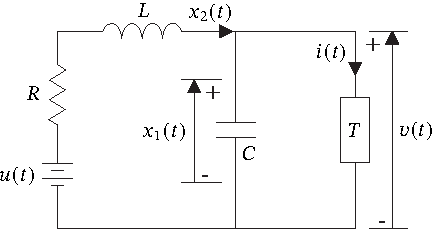
\includegraphics[scale=1]{circuito.pdf}\fonte{Elaborada pelo autor}}\hfill
%\captionbox{Gráfico da minipage\label{fig:minipage_grafico}}
%  [0.52\textwidth]{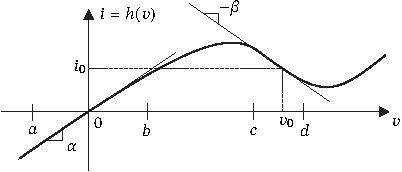
\includegraphics[scale=1.2]{diodocurva.pdf}\fonte{Elaborada pelo autor}}
%\end{figure}

\subsection{Subfiguras}

O pacote \textsf{subcaption} foi utilizado para inserir as \cref{fig:subfigura_circuito,fig:subfigura_grafico}. Para mais informações sobre o pacote, consulte seu manual\footnote{Disponível em: \url{https://mirrors.ctan.org/macros/latex/contrib/caption/subcaption.pdf}}.

\begin{figure}[htb]
\centering
\caption{Figura com subfiguras\label{fig:subfiguras}}
\subcaptionbox{Primeira subfigura\label{fig:subfigura_circuito}}
  {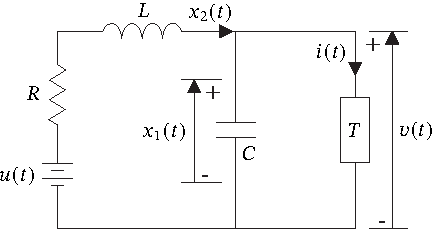
\includegraphics[scale=1]{circuito.pdf}} \hfill
\subcaptionbox{Segunda subfigura\label{fig:subfigura_grafico}}
  {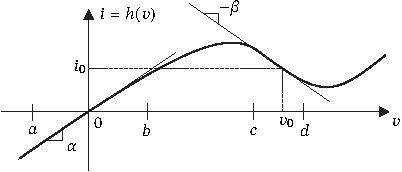
\includegraphics[scale=1.2]{diodocurva.pdf}}
\fonte{Elaborada pelo autor}
\end{figure}

%\begin{figure}
%\centering
% \caption{Figura com subfiguras}\label{fig:subfiguras}
% \begin{subcaptionblock}{0.47\textwidth}
%  \caption{Primeira subfigura}\label{fig:subfigura_circuito}
%  \centering
%  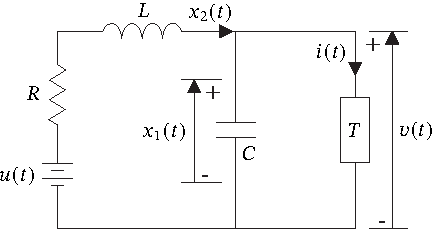
\includegraphics[scale=1]{circuito.pdf}
%\end{subcaptionblock}%
%\begin{subcaptionblock}{.52\textwidth}
%  \caption{Segunda subfigura}\label{fig:subfigura_grafico}
%  \centering
%  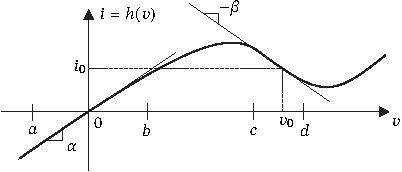
\includegraphics[scale=1.2]{diodocurva.pdf}
%\end{subcaptionblock}%
%\end{figure}

% ---
\subsection{Figuras que usam as mesmas fontes tipográficas do documento}
% ---

Para utilizar nas figuras as mesmas fontes tipográficas do texto, como na \cref{fig:psfrag1}, crie a figura \texttt{blockdiagram.eps}, mostrada na \cref{fig:psfrag2}. Softwares como InkScape, CorelDraw e Adobe Illustrator podem ser utilizados para esse fim.

\begin{figure}[htb]
\centering
\caption{Uso do pacote \textsf{psfrag}\label{fig:psgrag}}
\subcaptionbox{Arquivo \texttt{blockdiagram.pdf}\label{fig:psfrag1}}
  {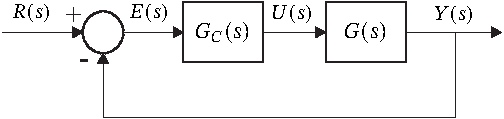
\includegraphics[scale=1]{blockdiagram.pdf}} \\ \medskip
\subcaptionbox{Arquivo \texttt{blockdiagram.eps}\label{fig:psfrag2}}
  {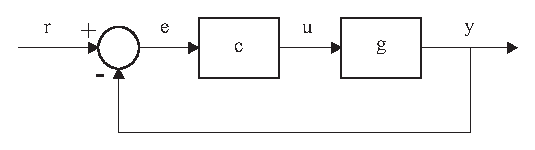
\includegraphics[scale=1]{blockdiagram.eps}}
\fonte{Elaborada pelo autor}
\end{figure}

Em seguida, crie um projeto auxiliar no Overleaf com o arquivo \texttt{blockdiagram.tex}, apresentado no \cref{cod:tex}, e defina-o como arquivo principal. Adicione ao projeto o arquivo \texttt{blockdiagram.eps}, compile-o com o compilador \texttt{LaTeX} e salve a figura gerada como \texttt{blockdiagram.pdf}. Esse arquivo poderá então ser utilizado no projeto principal, que é compilado com \texttt{pdfLaTeX}.

\lstinputlisting[float=htb,numbers=none,caption={\texttt{blockdiagram.tex}},label={cod:tex},fonte={Elaborado pelo autor}]{src/codigos/blockdiagram.tex}

Note que o \cref{cod:tex} utiliza o pacote \textsf{psfrag}, que permite substituir textos da figura original por conteúdos formatados com a mesma tipografia e os mesmos recursos matemáticos do documento. Por exemplo, o comando \verb|\psfrag{g}[c][c]{\small $G(s)$}| substitui ``g'' por ``$G(s)$''. Como o \textsf{psfrag} funciona apenas com o compilador \texttt{LaTeX}, o projeto auxiliar é uma forma simples de gerar figuras para documentos compilados com \texttt{pdfLaTeX}. Para mais detalhes, consulte o manual do pacote\footnote{Disponível em: \url{https://mirrors.ctan.org/macros/latex/contrib/psfrag/pfgguide.pdf}}.

Recomenda-se não utilizar arquivos \texttt{eps} diretamente no documento principal, pois o \texttt{pdfLaTeX} precisa convertê-los para \texttt{pdf}, o que aumenta o tempo de processamento.

% Capítulo de resultados
% ----------------------------------------------------------
\chapter{Ambientes do UnB\TeX}
% ----------------------------------------------------------

A classe UnB\TeX\ disponibiliza alguns ``ambientes'', ou seja, caixas de texto com formatação especial para certos tipos de elementos, que podem ser automaticamente numerados (por exemplo, \cref{def:WYSIWYG}, \cref{thm:WYSIWYG}, \cref{alg:ex}, etc.).

\section{Estilo teorema}

Criados com auxílio do pacote \textsf{mdframed}\footnote{Para mais informações, consulte: \url{https://mirrors.ctan.org/macros/latex/contrib/mdframed/mdframed.pdf}}, estão disponíveis os ambientes: \texttt{theorem}, \texttt{lemma}, \texttt{proposition}, \texttt{corollary}, \texttt{definition}, \texttt{as\-sumption}, \texttt{example}, \texttt{remark} e \texttt{proof}. Alguns exemplos de uso são apresentados a seguir.

\begin{definition}\label{def:WYSIWYG}
O WYSIWYG (ou ``What You See Is What You Get -- O que você vê é o formato final'') é um tipo de editor HTML que permite editar páginas web em uma visualização semelhante ao resultado final, sem necessidade de lidar diretamente com o código-fonte.
\end{definition}

\begin{theorem}[Teorema LaTeX--WYSIWYG]\label{thm:WYSIWYG}
    Todo físico prefere usar código \LaTeX\ puro que qualquer editor WYSIWYG.
\end{theorem}

\begin{proof}
    Físicos gostam de equações bonitas. Editores WYSIWYG não são apropriados para fazer equações bonitas\footnote{É certo que há editores WYSIWYG baseados em \LaTeX, mas eles não nos dão o mesmo nível de controle.}. Logo, se algum físico preferisse usar um editor WYSIWYG no lugar de \LaTeX, não seria muito inteligente. Como todo físico é inteligente, o teorema está demonstrado \textit{ad absurdum}.
\end{proof}

\begin{remark}\label{rmk:1}
    \LaTeX\ produz equações mais bonitas que qualquer editor WYSIWYG.
\end{remark}

%\begin{example}\label{exp:ae}
%    Einstein usaria um editor WYSIWYG ou \LaTeX? \\
%    Einstein era físico. Portanto, usando o teorema LaTeX-WYSIWYG, concluímos que ele usaria \LaTeX.
%\end{example}

Note que, por exemplo, o \cref{thm:WYSIWYG} é gerado pelo código:

\begin{verbatim}
\begin{theorem}[Teorema LaTeX--WYSIWYG]\label{thm:WYSIWYG}
    Todo físico prefere usar código \LaTeX\ puro que qualquer editor WYSIWYG.
\end{theorem}
\end{verbatim}

Caso queira definir um novo ambiente não disponibilizado no UnB\TeX, por exemplo, o ambiente \texttt{exercise}, acrescente os comandos a seguir:

\begin{verbatim}
\theoremstyle{definition}
\newmdtheoremenv[hidealllines=true,backgroundcolor=azulunb!10,innertopmargin=0pt]
    {exercise}{Exercício}[chapter]
\end{verbatim}

\theoremstyle{definition}
\newmdtheoremenv[hidealllines=true,backgroundcolor=azulunb!10,innertopmargin=0pt]{exercise}{Exercício}[chapter]
%\counterwithout{exercise}{chapter} % Numeração para o documento inteiro

\noindent O comando \verb|\theoremstyle{definition}| determina que o ambiente será numerado\footnote{Por padrão, a numeração do ambiente é feita por capítulo. Para numerar sequencialmente ao longo de todo o documento, adicione o comando \Verb{\counterwithout{exercise}{chapter}}}. A cor do ambiente é definida por \texttt{azulunb!10} (experimente também \texttt{verdeunb!10}). Com o novo ambiente definido, um exercício pode criado com os comandos:

\begin{verbatim}
\begin{exercise}\label{exc:in}
    Explique como Isaac Newton usaria cada um dos pacotes seguintes,
    se vivesse no tempo presente:
    \begin{enumerate}[label=(\alph*)]
        \item Metapost
        \item TikZ
        \item PGFPlots
        \item PSTricks
    \end{enumerate}
\end{exercise}
\end{verbatim}

\noindent O resultado é mostrado a seguir:

\begin{exercise}\label{exc:in}
    Explique como Isaac Newton usaria cada um dos pacotes seguintes,
    se vivesse no tempo presente:
    \begin{enumerate}[label=(\alph*)]
        \item Metapost
        \item TikZ
        \item PGFPlots
        \item PSTricks
    \end{enumerate}
\end{exercise}

Escreva \verb|exercício \ref{exc:in}| para se referir ao exercício \ref{exc:in} ou escreva apenas \verb|\cref{exc:in}| para que a palavra ``exercício'' e, não apenas o número correspondente, sejam gerados com hiperlink. No entanto, para que o comando \verb|\cref| funcione para o ambiente criado, no arquivo \texttt{tex} principal (\texttt{unbtex-example.tex}), antes do comando \verb|\begin{document}|, é necessário inserir os comandos

\begin{verbatim}
\crefname{exercise}{exercício}{exercícios}
\Crefname{exercise}{Exercício}{Exercícios}
\end{verbatim}

\section{Pseudocódigos}

O \cref{alg:ex} apresenta um exemplo de pseudocódigo elaborado com o pacote \textsf{algorithm2e}. Detalhes sobre seu uso podem ser encontrados em seu manual\footnote{Disponível em: \url{https://mirrors.ctan.org/macros/latex/contrib/algorithm2e/doc/algorithm2e.pdf}}. A lista de algoritmos pode ser incluída no trabalho por meio do comando \verb|\imprimirlistadealgoritmos| no arquivo \texttt{tex} principal.

\begin{algorithm}[htb]
\caption{Exemplo de pseudocódigo}\label{alg:ex}
\KwData{$n \geq 0$}
\KwResult{$y = x^n$}
$y \gets 1$\;
$X \gets x$\;
$N \gets n$\;
%\While{$N \neq 0$}{
\While(\tcc*[f]{Isso é um comentário}){$N \neq 0$}{
  \eIf{$N$ for par}{
    $X \gets X \times X$\;
    $N \gets \frac{N}{2}$ \tcc*[r]{Isso é outro comentário}
  }{\If{$N$ for ímpar}{
      $y \gets y \times X$\;
      $N \gets N - 1$\;
    }
  }
}
\fonte{Elaborado pelo autor}
\legend[Nota:]{Algoritmo inserido com o pacote \textsf{algorithm2e}}
\end{algorithm}

\section{Códigos-fonte}

O \cref{cod:exemplo} é um exemplo de código-fonte, inserido com auxílio do pacote \textsf{listings}. Para mais exemplos e comandos, confira o \cref{apd:cdg} e o manual do pacote\footnote{Disponível em: \url{https://mirrors.ctan.org/macros/latex/contrib/listings/listings.pdf}}. A lista de códigos é um elemento pré-textual não obrigatório de trabalhos acadêmicos e pode ser gerada e incluída utilizando-se o comando \verb|\imprimirlistadecodigos| no arquivo \texttt{tex} principal.

\begin{lstlisting}[float=htb,caption={Exemplo de código-fonte},label={cod:exemplo},fonte={Elaborado pelo autor},legend={Nota:}{Código inserido com o pacote \textsf{listings}}]
/**
* MSO: ativa o servo cujo eixo eh descrito
* por drive_axis; informacoes de controle
* sao gravadas em MSO_1
*/
  MSO(drive_axis,MSO_1);
/* Atribui o valor 0.0 ao primeiro elemento do array speed */
  speed[0] := 0.0; 
/* Atribui 1 para dataInitialized */
  dataInitialized := 1;
\end{lstlisting}

% Capítulo de conclusões
\include{src/capitulo5}

% ------------------------------------------------------------------------
% ELEMENTOS PÓS-TEXTUAIS
% ------------------------------------------------------------------------
\postextual

% ---
% Referências bibliográficas
% ---
\bibliography{src/referencias} % Arquivo com as referências bibliográficas
% ---

% ---
% Apêndices
% ---
\begin{apendicesenv}

% Imprime uma página indicando o início dos apêndices
\partapendices

% ----------------------------------------------------------
\chapter{Citações}\label{apd:cit}
% ----------------------------------------------------------

A classe UnB\TeX\ utiliza o pacote \texttt{unbtexcite} (derivado do \texttt{abntex2cite}, da classe abn\TeX2) para formatar citações e referências bibliográficas conforme as normas da ABNT. O arquivo \texttt{referencias.bib} contém exemplos de entradas bibliográficas que podem servir de modelo para a inclusão de novas referências em documentos. Os comandos a seguir podem ser utilizados para realizar citações:
\begin{verbatim}
\cite{nome_da_entrada}
\citeonline{nome_da_entrada}
\citeauthoronline{nome_da_entrada}
\citeyear{nome_da_entrada}
\end{verbatim}

Considere, por exemplo, a entrada do tipo manual (\texttt{@manual}) contida no arquivo \texttt{referencias.bib}:
\begin{verbatim}
@manual{memoir,
    address = {Normandy Park, WA},
    author = {Peter Wilson and Lars Madsen},
    organization = {The Herries Press},
    title = {The Memoir Class for Configurable Typesetting -- User Guide},
    url = {https://mirrors.ctan.org/macros/latex/contrib/memoir/memman.pdf},
    year = {2025}}
\end{verbatim}

Utilizando o comando \verb|\cite{memoir}| no arquivo \texttt{tex} correspondente a este parágrafo, o resultado gerado é \cite{memoir}. Para o comando \verb|\citeonline{memoir}|, o resultado gerado é \citeonline{memoir}. Os comandos \verb|\citeauthoronline| e \verb|\citeyear| apresentam separadamente no texto o nome dos autores e o ano da publicação. Por exemplo, podemos escrever:
\begin{mdframed}[style=plainSty,innertopmargin=8pt] % verde
Em \citeyear{memoir}, os autores \citeauthoronline{memoir} publicaram o manual da versão v3.8.4b do pacote \textsf{memoir}.
\end{mdframed}
O comando \verb|\footciteref{nome_da_entrada}| apresenta a referência como uma nota de rodapé. Todos os comandos de citação admitem argumento opcional para indicar uma posição específica da referência, como a página citada.

No arquivo \texttt{bib}, cada entrada de referência bibliográfica possuiu campos cujo preenchimento pode ser obrigatório ou opcional, a depender de seu tipo. No campo \texttt{author}, caso haja mais de um autor, seus nomes devem ser separados por \texttt{and}. Campos como \texttt{address}, \texttt{publisher} e \texttt{year} não preenchidos, podem gerar na lista de referências, respectivamente, as expressões abreviadas [\emph{s.l.}], [\emph{s.n.}] e [\emph{s.d.}] para indicar que são indeterminados. Recomenda-se o uso de programas gratuitos, como o JabRef\footnote{Disponível em: \url{https://www.jabref.org/}}, para auxiliar o preenchimento e gerenciamento de arquivos \texttt{bib}.

No arquivo \texttt{referencias.bib}, além da entrada para referência do tipo manual (como no exemplo dado), há também entradas para referências do tipo artigo de periódico \cite{greenwade1993}, artigo de conferência \cite{martin1997}, livro \cite{schaum1956}, capítulo de livro \cite{bates2010}, monografia \cite{morgado1990}, dissertação de mestrado \cite{macedo2005}, tese de doutorado \cite{guizzardi2005}, relatório técnico \cite{KBBDR2020}, dentre outras. Muitos outros exemplos podem ser encontrados em \cite{abntex2cite}.

Note que de acordo com as normas da ABNT, é obrigatório informar data para cada referência bibliográfica. Caso a data não seja identificada na referência, deve-se informar uma data aproximada entre colchetes, conforme situações ilustradas a seguir:

\begin{alineas}
    \item um ano ou outro: [2007 ou 2008]
    \item data provável: [2008?]
    \item data certa não indicada no item: [2008]
    \item use intervalos menores de 20 anos: [entre 1999 e 2008]
    \item data aproximada: [ca. 2000]
    \item década certa: [200-]
    \item década provável: [200-?]
    \item século certo: [20--]
    \item século provável: [20--?]
\end{alineas}

Em \citeonline{marins1991}, por exemplo, o ano provável é indicado por \citeyear{marins1991}. No arquivo \texttt{bib}, a entrada correspondente a esta referência tem o campo \texttt{year} declarado como \verb|year = {1991?}|.

Para mais informações sobre os comandos e o uso do \texttt{unbtexcite}, consulte os manuais do \texttt{abntex2cite} \cite{abntex2cite,abntex2cite-alf}, a partir do qual o \texttt{unbtexcite} foi derivado.

\include{src/apendice-b}

% ----------------------------------------------------------
\chapter{Códigos de programação}\label{apd:cdg}
% ----------------------------------------------------------

\section{Projeto do controlador por realimentação de estados}
\lstinputlisting[language=Matlab,caption={Código de Matlab},label={cod:matlab}]{src/codigos/controle.m}

\section{Exemplo de teste em malha fechada com entrada rampa}
\lstinputlisting[language=Python,caption={Código de Python},label={cod:python}]{src/codigos/controleSmithPredictor.py}

\section{Redução modal}
\lstinputlisting[language=Julia,caption={Código de Julia},label={cod:julia}]{src/codigos/ModalReduction.jl}

\end{apendicesenv}
% ---

% ---
% Anexos
% ---
\begin{anexosenv}

% Imprime uma página indicando o início dos anexos
\partanexos

\include{src/anexo-a}

\end{anexosenv}
% ---

\end{document}